\documentclass[12pt]{article}
\setlength{\textwidth}{17cm}
\setlength{\textheight}{24cm}
\setlength{\topmargin}{-2cm}
\setlength{\footskip}{1cm}
\setlength{\evensidemargin}{0cm}
\setlength{\oddsidemargin}{0cm}
\setlength{\parindent}{0cm}

\usepackage{allrunes}
\usepackage{amsmath}
\usepackage[magyar]{babel}
\usepackage[T1]{fontenc}
\usepackage[utf8]{inputenc}
\usepackage{fixltx2e}
\usepackage{multirow}

\usepackage[hyphens]{url}
\usepackage[unicode,colorlinks=true,breaklinks]{hyperref}
%\usepackage[dvips]{hyperref}
%should display links, but it does not work with \H accent
%and formulas in section titles

\hypersetup{colorlinks,linkcolor=blue,urlcolor=magenta,citecolor=magenta}
%Breaks long url`s in text, while keeping it one link:

\usepackage{amsfonts}
\usepackage{amsthm}
\usepackage{amssymb}


\theoremstyle{plain}
\usepackage{graphicx}

%\usepackage{gensymb}
\usepackage{float}

% For bra-ket notation
\usepackage{braket}

%% New commands
\newcommand{\dd}{\textrm{d}}

%% Pauli matrices
\newcommand{\sigx}{\sigma_x}
\newcommand{\sigy}{\sigma_y}
\newcommand{\sigz}{\sigma_z}

\newcommand{\paulix}{
    \left( \begin{array}{cc}
        0 & 1 \\
        1 & 0
    \end{array}
    \right)
}

\newcommand{\pauliy}{
    \left( \begin{array}{cc}
        0 & -i \\
        i & 0
    \end{array}
    \right)
}

\newcommand{\pauliz}{
    \left( \begin{array}{cc}
        1 & 0 \\
        0 & -1
    \end{array}
    \right)
}

% \begin{figure}[H]
%     \begin{center}
%     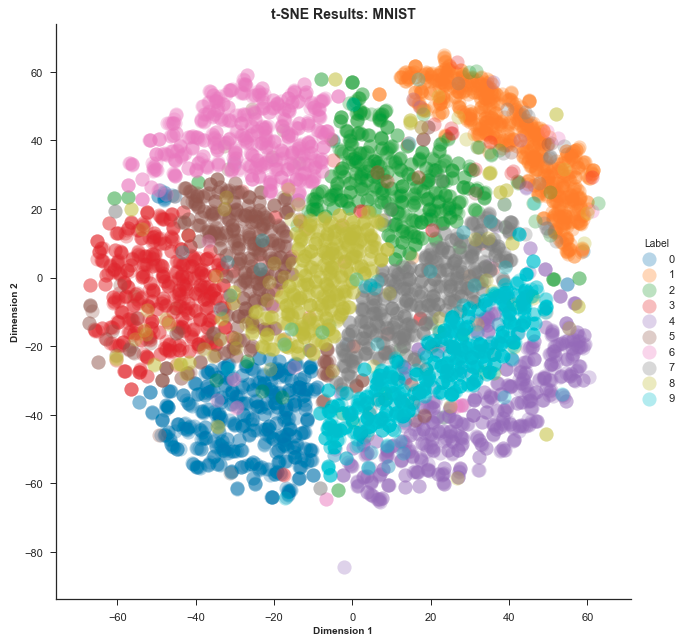
\includegraphics[width=0.5\textwidth]{media/tsneplot.png}
%     \caption{t-SNE plot for MNIST dataset \cite{tsne-article}} 
%     \label{fig:tsneplot}
%     \end{center}
% \end{figure}

\begin{document}
\title{\textbf{11. tétel}}
\author{Berekméri Evelin}


\maketitle

\pagenumbering{gobble}

\vspace{9cm}
\tableofcontents

\newpage
\begin{abstract}

Számítógépes tanulás – Predikciós és klasszifikációs módszerek. Felügyelt és felügyelet nélküli tanítás. A tanítóhalmaz, a validáció és a túlfittelés. K-means, Support Vector Machine, Random Forest, k-NN-módszer.
\end{abstract}

\section{Számítógépes tanulás}
A gépi tanulás a mesterséges intelligencia egy ága. Olyan módszereket foglal magába, amelyek meglévő adatokból építenek matematikai modelleket ahhoz, hogy szabályszerűségeket ismerjenek fel vagy predikciókat hajtsanak végre - ismeretlen adatokra is. A gépi tanulásos algoritmusokat két nagy csoportra oszthatjuk: felügyelt (supervised) és felügyelet nélküli tanításra (unsupervised learning). Felügyelt tanítás esetén a statisztikai modell "input" adatok alapján prediktál "output" adatokat. A felügyelet nélküli tanítás tárgykörébe tartozó módszerek esetén nem beszélhetünk output adatokról, ugyanis az algoritmus a rendelkezésre álló adathalmaz szerkezetéről és kapcsolatairól szolgál többletinformációval. 

\section{Felügyelt tanítás}
A felügyelt tanítás esetén használt adathalmazban minden megfigyelés esetén az input éték(ek)hez tartozik egy output érték. Az input változókat általában X-szel jelöljük ($X = (X_1, X_2, ..., X_p) $ p db változó esetén) és többféleképpen szoktak rá hivatkozni:  (független) változók - (independent) variables -, "features", "predictors". Az ouput változókat - másnéven függő változókat (dependent variables) vagy válaszokat - általában Y-nal jelöljük. Azt feltételezzük, hogy az X és az Y között van valamilyen kapcsolat, amelyet a következőképpen írhatunk fel: $$ Y = f(X) + \epsilon,$$ ahol $f$ X ismeretlen függvénye és $\epsilon $ a hiba tag, amely független X-től és az átlaga nulla. $f$ becslése predikció vagy inferencia végrehajtásához szükséges. 

A gépi tanulás és a statisztikai tanulás fogalma gyakran összemosódik az emberek fejében, viszont bizonyos források szerint a lényeges különbség a két terület között az a céljük: a gépi tanulás helyes predicióra fókuszál, ezzel ellentétben a statisztikai tanulás célja az X és Y közötti kapcsolat felderítése (inferencia). 

\subsection{Predikció}
Sok esetben az X inputhalmaz könnyen elérhető, de az Y nem könnyen hozzáférhető. Ilyenkor, mivel a hibatag nullára átlagolódik, megjósolhatjuk Y-t: $$ \hat{Y} = \hat{f}(X), $$ ahol $\hat{f}$ f becslése és $\hat{Y}$ Y becsült értéke. $\hat{f}$-et ilyenkor többnyire fekete dobozként kezeljük, mivel általában nem ismerjük annak egzakt formáját. $\hat{Y}$ pontossága két tényezőtől függ: a reducibilis és az irreducibilis hibától. Általában $\hat{f}$ nem becsli elég jól $f$-et, ezért ebből is származik egy hiba. Viszont ez a hiba reducibilis, mivel $\hat{f}$ pontosságát tudjuk növelni pontosabb módszerekkel. Ugyanakkor, ha teljes pontosan meg is tudnánk határozni f-et, a megbecsült válasznak $\hat{Y} = f(X)$ formája lenne és ez még így is tartalmazna hibát, mivel Y $\epsilon$ függvénye is, amit viszont nem lehet X-ből meghatározni. Tehát $\epsilon$ variabilitása is hatással van a predikció pontosságára. Ezt irreducibilis hibának nevezik, mivel akármennyire is pontosan becsüljük meg f-et, nem tudjuk csökkenteni az $\epsilon$ miatt megjelenő hibát. $\epsilon$ magába foglalhat meg nem mérhető tényezőket, illetve olyan meg nem mért változókat, amelyek hasznosak lehetnek Y predikciójában. Ilyenkor Y megbecsült és valódi értéke közötti különbség négyzetének várható értéke a következőképpen áll elő: $$ E[Y-\hat{Y})^2= E(f(X)+\epsilon-\hat{f(X)}]^2=[f(X)+\hat{f(X)}]^2 + Var(\epsilon), $$ ahol $Var(\epsilon) $ $\epsilon$ szórása. Az első tag reducibilis és a második tag az irreducibilis hibát jelöli. %A cél az, hogy csökkentsük a reducibilis hibát. 
Az irreducibilis hiba egy felső határt jelöl ki Y becslésének pontosságára. 

\subsection{Inferencia}
Inferencia esetén f egzakt formáját keressük, mivel a célunk nem feltétlenül az, hogy prediktáljunk vele, hanem az, hogy jobban megértsük a kapcsolatot X és Y között (Y hogyan változik X függvényében). Olyan kérdésekre keressük ilyenkor a válasz, mint például:  
\begin{itemize}
    \item mely input változók vannak ténylegesen kapcsolatban az output értékkel?
    \item milyen kapcsolatban állnak az input változók az output értékkel? mely változók növekedésének hatására növekszik az output, melyekre csökken?
    \item milyen formában írható fel a kapcsolat az input és az output között? pl. lineáris? 
\end{itemize}

\subsection{f becslése}
Különböző lineáris és nem lineáris módszerek léteznek f megbecslésére. A rendelkezésünkre álló adathalmaznak azt a részét, amelyen betanítjuk a modellünket f megbecslésére, tanító (training) adathalmaznak nevezzük. Ha van n db megfigyelésünk és p db független változónk, ugyanakkor $x_{ij}$ jelöli az x-edik "sorban" levő megfigyeléshez tartozó, j-edik "oszlopban" levő független változót (i = 1, 2, ..., n és j = 1, 2, ..., p), illetve $y_i$ jelöli az i-edik megfigyeléshez tartozó outputot, akkor a training adathalmazunkat a következőképpen írhatjuk fel: $$ \{(x_1, y_1), (x_2, y_2), ..., (x_n, y_n)\}, $$ ahol $$ x_i = (x_{i1}, x_{i2}, ..., x_{ip})^T.$$ A cél az, hogy olyan f függvényt találjunk, ami Y-t a lehető legjobban megközelíti, azaz a reducibilis hibát a lehető legjobban csökkenti ($\hat{Y} \proportional \hat{f}(X).$ Ehhez különböző paraméteres és nem paraméteres módszerek léteznek. A paraméteres módszerek esetén rögzítjük, hogy f-nek milyen formát feltételezünk (pl. lineárisan függ a független változóktól: $ f(X) = \beta_0 + \beta_1 X_1 + ... + \beta_p X_p $) és valamilyen módszerrel (pl. legkisebb négyzetek módszerével) fitteljük a függvényt a megfigyelési adatokra, amivel megkapjuk a $\beta_i$ együtthatókat. Ez magában hordozza annak a kockázatát, hogy f valójában nagy mértékben különbözik attól a formától, amit mi feltételeztünk. Ehhez képest a nem paraméteres módszerek esetén nem teszünk explicit feltételezéseket f formájáról, nem áll fenn a veszélye, hogy a rosszul feltételezett függvény forma miatt nem lesz elég pontos $\hat{f}$, viszont ugyanakkor sokkal több megfigyelésre van szükségünk, mint a paraméteres módszereknél. Ha a célunk az inferencia, ajánlott a kevesebb változót számításba módszereket választani, mivel ezeket könnyebb értelmezni, ezek viszont általában kevésbé flexibilisek a nem-paraméteres módszerekhez képest, amelyeket érdemes inkább akkor választani, ha prediktálni szeretnénk a modellel. 

Egy további szempont szerint az adathalmazt két csoportba osztjuk aszerint, hogy kvantitatív vagy kvalitatív adatokat tartalmaznak. A kvantitatív változók numerikus értékeket vesznek fel. A kvalitatív változók K db különböző osztály (kategória) közül vesznek fel egy értéket. Abban az esetben, ha a függő változóink kvantitatívak, regressziót alkalmazunk. Kvantitatív output esetén klasszifikációt hajtunk végre. Ugyanakkor bizonyos esetekben a klasszifikációra is tekinthetünk regresszióként, ha osztály valószínűségeket prediktálunk konkrét osztály helyett. 

\subsection{Klasszifikáció}


Klasszifikáció során tehát kvalitatív válaszokat prediktálunk, amelyek egy véges halmazból vesznek fel értékeket. Ilyen módszer például a logisztikus regresszió, a lineáris diszkriminancia-analízis, a KNN, a döntési fa, a random forest, a boosting és a support vector machine. Felmerülhet a kérdés, hogy miért nem alakítjuk át a válaszokat numerikus értékké és alkalmazunk rajtuk regressziós módszereket. Ez azért nem egy járható út, mivel azt feltételezi, hogy létezik egy bizonyos sorrend a kategóriák között. Például, ha az A, B, C kategóriákat 1, 2, 3 számoknak feleltetjük meg, akkor azt feltételezzük, hogy ugyanakkora a "távolság" A és B között, mint a B és C között. Ugyanakkor megválaszthatjuk az átalakítást másféleképpen is, pl.  A=3, B=2 és C=1. Erre viszont különböző modellt kapnánk lineáris regresszióval. Ez a módszer csak akkor működik, ha a kategóriák sorba állíthatók (pl. kis, közepes, nagy) és a kategóriák közötti "különbség" azonos vagy ha csak két kategória van - bináris/kétszintű válaszok esetén a két lehetséges kódolás bármelyikére ugyanazt az eredményt kapjuk. 


\subsection{K-Nearest Neighbors}
\subsubsection*{KNN klasszifikáció}
\begin{figure}
    \begin{center}
    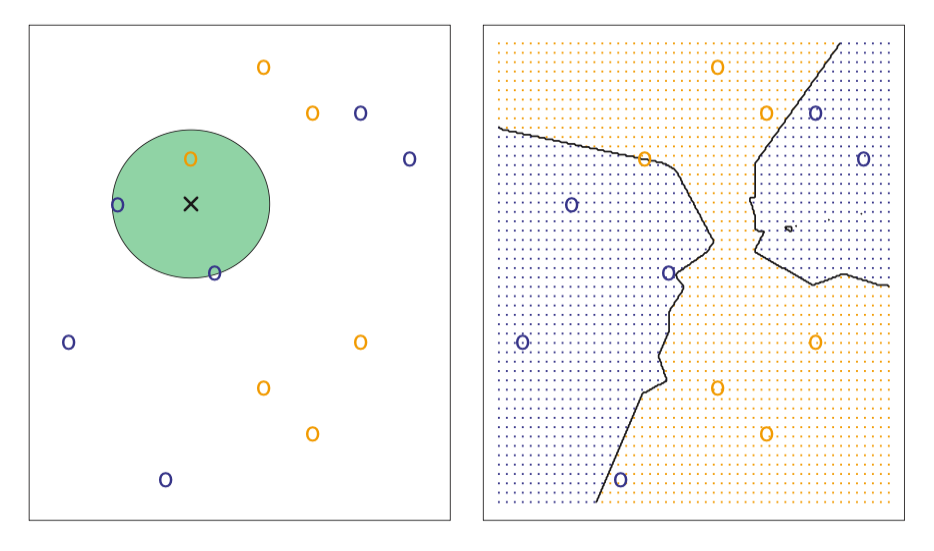
\includegraphics[width=0.8\textwidth]{media/knn1.png}
    \caption{KNN megfigyelés K = 3 esetén. A próba megfigyelést, amelyre meg szeretnénk határozni, hogy melyik kategóriába tartozik, a fekete x jelöli (bal oldal). A tanítóhalmaz 6 db kék és 6 db narancssárga osztályhoz tartozó adatot tartalmaz. A kör a kijelölt ponthoz legközelebb eső 3 szomszédot veszi körül, két kék és egy narancssárga pontot. A leggyakrabban előforduló kategória a kijelölt pont K db szomszédja között tehát a kék, így a KNN azt prediktálja, hogy a kijelölt pont is a kék osztályhoz tartozik. A jobb oldali képen látható a döntési határ fekete vonallal, amely elhatárolja, hogy a teszt pontok mely kategóriába lesznek sorolva annak függvényében, hogy a narancssárga vagy a kék területen helyezkednek el. } 
    \label{knn1}
    \end{center}
\end{figure}

A K-Nearest Neighbors (KNN) klasszifikáció egy olyan módszer, amely a megfigyelések szomszédos pontjainak outputjából jósolja meg, hogy a megfigyelések melyik kategóriába tartoznak.  A KNN Y X szerinti feltételes valószínűségét becsli és osztályozza a megfigyeléseket a legmagasabb becsült valószínűség szerint: 
$$ Pr(Y=j | X = x_0) = \frac{1}{K} \sum_{i \in N_o} I(y_i = j), $$ ahol $Pr(Y=j | X = x_0) $ jelöli annak a valószínűségét, hogy a megfigyelés a j kategóriába esik feltéve, ha a szóban forgó megfigyelés éppen $x_0$, K a számításba vett szomszédok száma (egész szám), $N_0 $ $x_0$-hoz legközelebb levő K db szomszédos megfigyelés halmaza, I pedig egy indikátor változó, amelynek 1 az értéke, ha y a j kategóriába tartozik és 0 ellenkező esetben. Ezután a KNN abba a kategóriába rendeli a megfigyelést, amelynek legnagyobb a valószínűsége. A KNN működését a \ref{knn1} ábra szemlélteti. 
%a Bayes-szabályt alkalmazza és

\begin{figure}
    \begin{center}
    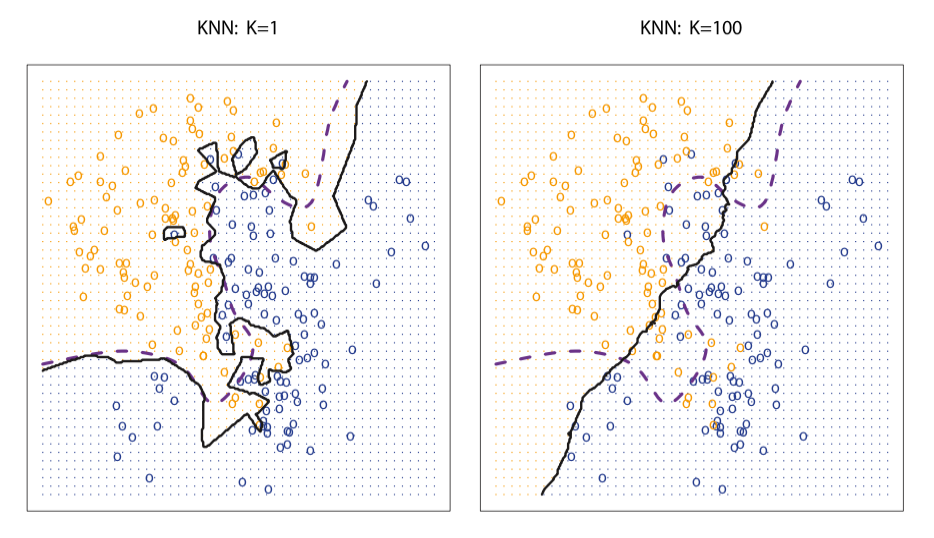
\includegraphics[width=0.8\textwidth]{media/knn2.png}
    \caption{Döntési határok összehasonlítása K=1 és K=100 esetén (fekete folytonos vonalak) az elméleti modellel (szaggatott vonal). A döntési határ az első esetben túl flexibilis, a második esetben pedig nem elég flexibilis. } 
    \label{knn2}
    \end{center}
\end{figure}

K megválasztása nagy hatással van az osztályozásra. K=1 esetén a döntési határ túl flexibilis és túlérzékeny a mintázatra. K növekedésével a módszer flexibilitása csökken és a lineárist egyre inkább megközelítő döntési határt produkál (\ref{knn2} és \ref{knn3} ábra). 

\begin{figure}
    \begin{center}
    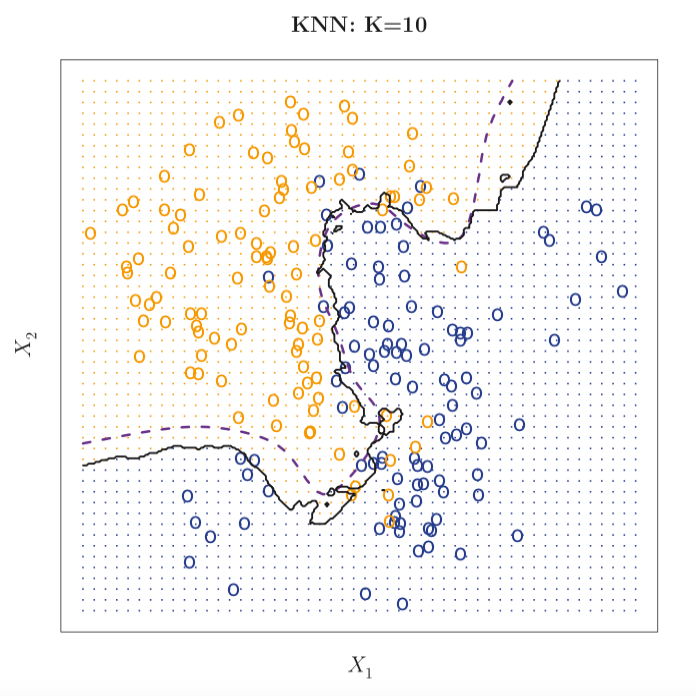
\includegraphics[width=0.5\textwidth]{media/knn3.png}
    \caption{K=10 esetén prediktált döntési határ (folytonos fekete vonal) összehasonlítása az elméleti határral (szaggatott vonal). } 
    \label{knn3}
    \end{center}
\end{figure}

\subsubsection*{KNN regresszió}
A KNN regresszió hasonlóan működik, mint a KNN klasszifikáció, viszont kategóriák helyett numerikus értékeket prediktál minden megfigyelés esetén: $$ \hat{f}(x_0)=\frac{1}{K} \sum_{i \in N_o} y_i.$$ 

A KNN módszer egy nem-paraméteres módszer, tehát semmilyen feltételezést nem teszünk a döntési határ alakjáról. 


\subsection{Random Forest}
\subsubsection{Fa alapú módszerek}
A fa alapú módszerek a predictor teret felosztják kisebb részekre. Ahhoz, hogy predikciót hajtsunk végre egy megfigyelésre, általában átlagot vagy módust számolunk (az adathalmaz annak a részének az átlagát/módusát, amelyhez a megfigyelés tartozik). A fa alapú módszereket könnyen lehet értelmezni, de legtöbbször nem veszik fel a versenyt a legjobb felügyelt tanításos algoritmusokkal a predikciók pontosságának szempontjából. Vannak olyan módszerek, amelyek több fát egyesítenek a predikcióhoz, pl. bagging, random forests és boosting. A fák egyesítése növeli a predikció pontosságát a modell értelmezhetőségének kárára. A döntési fák alkalmazhatók regresszióra és klasszifikációra is. 

A \ref{tree1} és \ref{tree2} ábrákon egy példa látható, amelyen baseball játékosok fizetése kerül megbecslésre aszerint, hogy mekkora a régiségük ("Years") és hány találatuk volt ("Hits"). A \ref{tree1} ábra szerint, az átlagfizetése azoknak, akiknek 4.5 évnél kevesebb tapasztala van, 5.11 dollár (logaritmikus skálán). Tehát, ha van egy megfigyelésünk, ami szerint egy játékosnak pl 3 év tapasztala van, akkor az lesz a predikciónk, hogy a játékos fizetése 5.11. Akiknek 4.5 évnél több tapasztalatuk van, újabb elágazás van a találatok számának átlagánál. A fának vannak terminális nodejai (levelek) és belső nodejai. A példa szerint az éves tapasztalat a legfontosabb szempont a fizetés meghatározásában. A kevesebb tapasztalattal rendelkező játékosok kevesebbet keresnek és nem játszik nagy szerepet a fizetésükben az, hogy hány találatuk volt. 

Az a cél tehát, hogy J db diszjunkt, $R_J$ részre osszuk fel a tanítóhalmaz terét úgy, hogy az $$ RSS = \sum_{j=1}^J \sum_{i \in R_j} (y_i - \hat{y_{R_j}})^2$$ minimális legyen, ahol $\hat{y_{R_j}}$ az átlagos output a j-edik részben ("dobozban"). Minden megfigyelésre, ami a $R_J$ részbe esik, ugyanazt prediktáljuk, ami tulajdonképpen az átlaga a $R_J$-ben levő tanítóadat outputjainak. Az, hogy a tanítóhalmaz minden lehetséges felosztására ellenőrízzük az RRS-t nagyon számításigényes lenne, ezért top-down, greedy megközelítést alkalmazunk, vagyis rekurzív bináris felosztást. Azért greedy (mohó), mert minden lépésnél csak arra a lépésre nézve lesz kiválasztva a legjobb szétágazás, nem a teljes fára nézve. 
Tehát a rekurzív bináris szétválasztásban választunk egy $X_j$ predictort és egy $s$ vágási pontot úgy, hogy a predictor tér $R_1(j, s)=\{X/X_j<s\}$ és $R_2(j, s)=\{X/X_j >= s\}$ része minimalizálja RSS-t. Vagyis végigmegyünk az összes $X_j$ és $s$ lehetséges értékén és azt a párt válasszuk ki, amelyre $$ \sum_{j: x_i \in R_1} (y_i - \hat{y_{R_1}})^2 + \sum_{i: x_i \in R_2} (y_i - \hat{y_{R_2}})^2 $$ minimimális. A következő szinten, a predictor és az elágazási érték keresése esetében hasonlóképpen járunk el, csak ahelyett, hogy a teljes predictor teret választanánk ketté, a két már azonosított $R_1, R_2$ részt választjuk tovább szét. A folyamatot addig folytatjuk, ameddig bizonyos kritérium teljesül, pl egyik rész sem tartalmaz 5 megfigyelésnél többet. 

Ez a módszer jó predikciókat eredményezhet a tanítóhalmazon, viszont esélyes, hogy túltanítjuk, ha a fa túl bonyolult lesz. Egy egyszerűbb fa, kevesebb elágazodással jobban is értelmezhető. Az egyik lehetséges módszer a túlbonyolítás elkerülésére az, hogy csak addig folytatjuk az újabb elágazodások létrehozását, ameddig az RSS csökkenés egy bizonyos határérték fölött marad. Ennek az a hátránya, hogy túl rövidlátó, mivel lehet, hogy egy kis RSS csökkenés után lennének még fontos elágazódások. A másik módszer egy hosszú fa létrehozása és annak visszametszése egy alfára. Az alfa kiválasztásakor az RSS-hez hozzáadjuk a levelek számát megszorozva egy paraméterrel, és ezt az összeget minimalizáljuk. Ezzel a paraméterrel hangolható a levelek számának költsége. 

A klasszifikációs fák hasonlóak a regressziós fákhoz, viszont a $R_i$ részhez tartozó tanítóadatok átlagos outputja helyett azt prediktálja, hogy melyik a leggyakrabban előforduló osztály. Ezért nem RSS használatos a rekurzív bináris szétágazáskor, hanem olyan értékek, amelyek tartalmazzák azoknak az adatoknak az arányát egy adott $R_i$-ben, amelyek nem a legyakoribb osztályhoz tartoznak (klasszifikációs hiba ráta, Gini-index, entrópia). 

A fa alapú módszerek előnyei: könnyen értelmezhetők, jobban imitálják az emberi döntéshozatalt, grafikusan könnyen ábrázolhatók, könnyen kezelik a kvalitatív prediktorokat anélkül, hogy numerikussá kellene őket változtatni. Hátrányai: alacsonyabb predikciós pontosság, robosztusság hiánya az adatok változására. Több fa egyesítésével lehet növelni a predikció pontosságát. 


\begin{figure}
    \begin{center}
    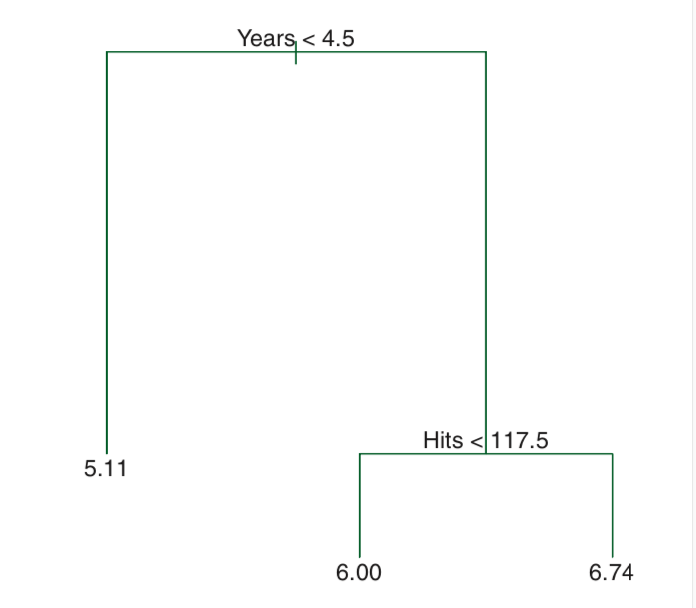
\includegraphics[width=0.7\textwidth]{media/tree1.png}
    \caption{Regresszió fára példa, 2 predictor szerint.} 
    \label{tree1}
    \end{center}
\end{figure}

\begin{figure}
    \begin{center}
    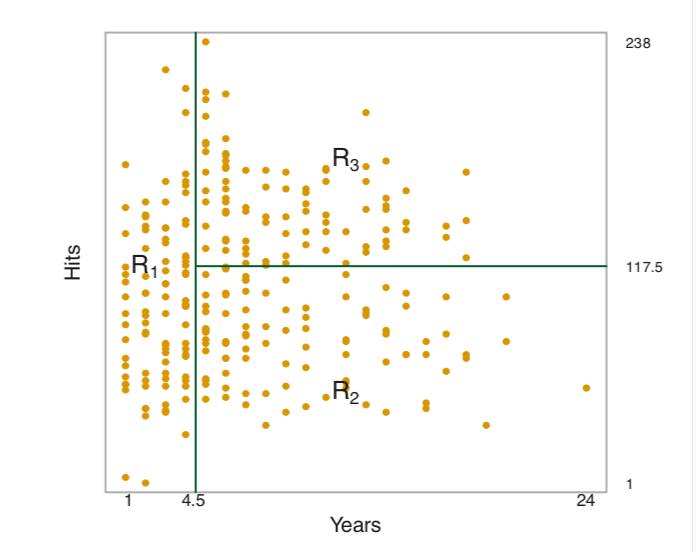
\includegraphics[width=0.7\textwidth]{media/tree2.png}
    \caption{Az adathalmaz felosztása a döntési fa szétágazásai szerint. } 
    \label{tree2}
    \end{center}
\end{figure}

\subsubsection{Bagging}
A random forest értelmezéséhez érdemes megérteni a bagging lényegét előbb. Az eddig említett döntési fák nagy szórással prediktálnak. Vagyis, ha random kétfelé osztjuk a tanítóhalmazt, két meglehetősen különböző fát kapunk a két adathalmazra. A bagging, vagyis a bootstrap aggregation egy általános módszer statisztikai tanulásos módszerek szórásának csökkentésére, amelyet gyakran alkalmaznak döntési fákra is. Az átlagolás egy általános módszer a szórás csökkentésére (az átlag szórásnégyzete $\sigma^2/n$, ha az egyes adatok szórása $\sigma^2$). Bagging esetén bootsrap-et használunk, azaz a tanítóhalmazból B darab bootstrappelt adathalmazt generálunk, mindegyik halmazon tanítjuk a modellünket és a végén átlagolj a B db predikciót: 
$$ \hat{f_{bag}} = \frac{1}{B} \sum_{b=1}^B\hat{f*^b}(x). $$
Klasszifikáció esetén a leggyakrabban előforduló válasz a bagging prediktált értéke. A bagging jelentősen növeli a predikció pontosságát, viszont csökkenti a modell értelmezhetőségét. 

\subsubsection{Random Forests}
A random forests egy javítása a bagged fáknak, amely dekorrelálja a fákat. Ebben az esetben is több döntési fát tanítunk be bootstrappelt tanítóhalmazon, viszont egy elágazás létrehozásánál nem az összes p db predictor, hanem csak m <= p db predictort veszünk számításba (tipikusan $m=\sqrt{p}$). Ez azért van, mert ha van egy nagyon erős predictor kevésbé erősebb predictorok között, akkor valószínű, hogy az összes fa azt fogja választani, így korreláltak lesznek a modellek. Sok korreláló adat átlagolása nem vezet akkora szóráscsökkentéshez, mint nem korreláló adatok esetén. H m egyenlő p-vel, akkor visszatérünk a  bagginghez.

\subsection{Support Vector Machine}
\begin{figure}
    \begin{center}
    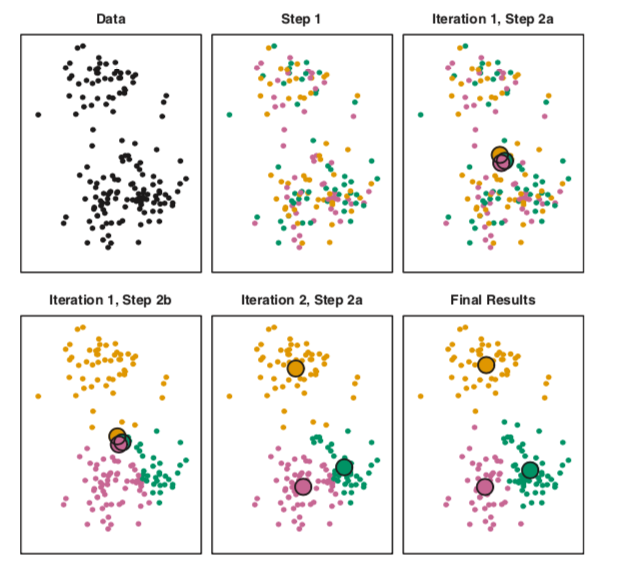
\includegraphics[width=1\textwidth]{media/kmeans.png}
    \caption{} 
    \label{kmeans}
    \end{center}
\end{figure}
A Support Vector Machine (SVM) egy hatékony predikciós módszer, melyet főleg bináris klasszifikáció használnak. Egy lineáris függvény képezi a módszer alapját: 
$ \textbf{w}^T\textbf{x}+\textbf{b}. $ Ha ez az érték pozitív a megfigyelés az egyik osztályhoz, ha negatív, a másik osztályhoz tartozik. Ez a lineáris függvény egy hipersíktól való távolság mértékével azonosítható, egy döntési határértékkel eltolva. A $$ \textbf{w}^T\textbf{x}+\textbf{b}=\textbf{b}+\alpha_i \textbf{x}^T \textbf{x}^{(i)}$$ egy kernel trükköt foglal magába, ami megengedi, hogy a bal oldalon levő lineáris függény a jobb oldali formába legyen írva, ahol $w^T$ a hipersíkra merőleges vektor, $x$ a minta poziciója, $x^{(i)}$ egy tanítóadat és $\alpha$ egy együttható vektor. Ez az átírás megengedi, hogy az \textbf{x}-et helyettesítsük egy feature függvénnyel ($\phi(\textbf{x})$) és a skaláris szorzatot egy $k(\textbf{x, x}(i)) = φ(\textbf{x}) \dot φ(\textbf{x(}i))$ függvénnyel, amit kernelnek hívunk.  Ezután a predikciókat végezhetjük az $$ f(x)= b + \sum_i \alpha_i k(\textbf{x, x}(i)),$$ ami nem lineáris \textbf{x}-ben, de a kapcsolat $\phi(\textbf{x}) $ és $f(\textbf{x})$ között, illetve $\alpha$ és $f(\textbf{x}) $ között lineáris. A kernel alapú módszer ekvivalens azzal, mintha feldolgozás előtt alkalmaznánk az input adatokra egy $\phi(\textbf{x})$ függvényt, majd egy lineáris modellt tanítanánk be a transzformált térben. Ennek a módszernek az előnyei, hogy betaníthatók olyan adatokra, amelyek nem linárisak x függvényében, konvex optimalizáló technikákat haasználva és mert a kernel függvény hatékonyabb, mint két $\phi(\textbf{x}) $ vektor szorzatát kiszámolni. 



\section{Felügyelet nélküli tanítás}
A felügyelet nélküli tanítás során nem állnak rendelkezésre output adatok, amivel "felügyelnénk", ellenőrízhetnénk a tanulás minőségét, hanem az adathalmazunk belső szerkezetéről, kapcsolatairól tudhatunk meg többet. Ilyen algoritmus például a klaszterezés, amely különböző osztályokba sorolja az adatoka. 

\subsection{K-mean klaszterezés}
K-means klaszterezés alkalmazásakor először meg kell adnunk K értékét, azaz hogy hány osztályba szeretnénk sorolni az adatokat. Az algoritmus minden adatot pontosan egy klaszterbe tesz. A klaszterek nem fednek át, tehát particionálják az adathalmazt. Az számít jó klaszterezésnek, amelynek a teljes "within-cluster variation" értéke alacsony ($W(C_k)$): $$minim \{sum_k{k=1}^K W(C_k)\}$$ minden $C_k$-ra, amelyek a különböző klasztereket jelölik. A legáltalánosabb módszer $W(C_k))$ választására a négyzetes euklidészi távolság: $$ W(C_k)=\frac{1}{|C_k|} \sum_{i, i¨ \in C_k} \sum_{j=1}^p (x_{ij} - x_{i¨j})^2, $$ ahol $|C_k|$ a megfigyelések számát jelöli egy bizonyos klaszterben. 
A K-mean klaszterezés algoritmus lépései:
\begin{enumerate}
    \item Először minden megfigyeléshez rendelünk egy számot 1-től K-ig, azaz besoroljuk valamelyik osztályba. Ez az inicális klaszterezés. 
    \item Iteráljuk addig, ameddig a klaszterezés nem változik többet: minden K klaszterhez számoljuk ki a klaszter centroidját. A centroid egy p hosszú vektor, amely tartalmazza a p darab feature átlagát az adott klaszterben. Majd rendeljük hozzá minden megfigyelést ahhoz a klaszterhez, amelynek a centroidja a legközelebb van (a távolságot euklideszi távolsággal számoljuk ki). 
\end{enumerate}
Az algoritmus lépéseit a \ref{kmeans} ábra ábrazolja. 



A kidolgozás többnyire a \cite{minden} könyv szerint készült. 

\begin{thebibliography}
%\bibitem{wiki_ml}
%\url{https://hu.wikipedia.org/wiki/G%C3%A9pi_tanul%C3%A1s}

\bibitem{minden}
Gareth James, Daniela Witten, Trevor Hastie, Robert Tibshirani, An Introduction to Statistical Learning with Applications in R, Springer, 2017

%Predicting chemical properties of molecules from their wavefunctions using spherical convolutional neural network, Biricz András


\end{thebibliography}

\end{document}